\documentclass[english]{beamer}
 
\usepackage[english]{babel}
\usepackage[T1]{fontenc}
\usepackage[utf8]{inputenc}
\usepackage{upgreek}
\usepackage{amsmath}
\usepackage{amssymb}
\usepackage{pdfpages}
\usepackage[]{algorithm2e}
\usepackage[abs]{overpic}
\usepackage{mdwlist}
\usepackage{tikz}
\usepackage{hhline}
\usepackage{tikz}
\usepackage{subcaption}
\usepackage{tikz-qtree}
\usepackage{pbox}
\usepackage{forest}
\usepackage{slashbox}
\usepackage{hhline}
\usepackage{colortbl}
\usepackage{array}

\usetikzlibrary{trees}
\usetikzlibrary{babel}
\usetikzlibrary{arrows,automata,positioning}

\usepackage[style=alphabetic,backend=bibtex,autocite=footnote]{biblatex}

% \bibliographystyle{alpha}
\bibliography{biblio.bib}
\nocite{*}

\usetheme{Frankfurt}
  
\title{Phylogeny of JPEG images by ancestor estimation using missing markers on image pairs}
\author{Noé Le Philippe, William Puech and Christophie Fiorio}
\institute{LIRMM Laboratory, CNRS, University of Montpellier, France}
\date{\today}
% \logo{\includegraphics[height=10mm]{images/logo.png}}

\addtobeamertemplate{navigation symbols}{}{%
    \usebeamerfont{footline}%
    \usebeamercolor[fg]{footline}%
    \hspace{1em}%
    \insertframenumber/\inserttotalframenumber
}

\AtBeginSection[]
{
  \ifnumcomp{\value{section}}{=}{1}{}
  {
    \begin{frame}
      \frametitle{Table of content}
      \tableofcontents[currentsection, hideothersubsections]
    \end{frame}
  }
}

\makeatletter
\renewcommand\@makefnmark{\hbox{\@textsuperscript{\normalfont[\@thefnmark]}}}
\renewcommand\@makefntext[1]{{\normalfont[\@thefnmark]}\enspace #1}
\makeatother

\DeclareCiteCommand{\footfullcitetext}[\mkbibfootnotetext]
{\usebibmacro{prenote}}
{\usedriver
  {\DeclareNameAlias{sortname}{default}}
  {\thefield{entrytype}}}
{\multicitedelim}
{\usebibmacro{postnote}}

\newcolumntype{L}[1]{>{\raggedright\let\newline\\\arraybackslash\hspace{0pt}}m{#1}}
\newcolumntype{C}[1]{>{\centering\let\newline\\\arraybackslash\hspace{0pt}}m{#1}}
\newcolumntype{R}[1]{>{\raggedleft\let\newline\\\arraybackslash\hspace{0pt}}m{#1}}

\newenvironment<>{varblock}[2][.9\textwidth]{%
  \setlength{\textwidth}{#1}
  \begin{actionenv}#3%
    \def\insertblocktitle{#2}%
    \par%
    \usebeamertemplate{block begin}}
  {\par%
    \usebeamertemplate{block end}%
  \end{actionenv}}

\begin{document}
\selectlanguage{english}
\begin{frame}
  \titlepage
\end{frame}

\section{Introduction}
\begin{frame}
  \frametitle{What is image phylogeny}

  \begin{block}{Definition}
    {\large ``In biology, phylogenetics is the study of evolutionary history and relationships among individuals or group of organisms''}
    \hspace*\fill{\small--- Wikipedia}
  \end{block}
  \pause
  
  \begin{block}{For images}
    The study of evolutionary history and relationships among images
  \end{block}
\end{frame}

\begin{frame}
  \frametitle{What is image evolution}

  \begin{block}{Near duplicates\footnotemark}
    $I_{n+1} = T(I_{n}),\ T \in \mathcal{T}$
  \end{block}
  \pause
  \begin{block}{Tolerated transformations}
    \begin{itemize}
    \item transformations in $\mathcal{T}$
    \item magnitude of the transformation
    \end{itemize}
  \end{block}
  \pause
  \begin{block}{Our goal}
    Compute an image phylogeny tree of near duplicates where $\mathcal{T} = \{lossy\ compression\}$
  \end{block}
  \footfullcitetext{joly2007content}
\end{frame}

\begin{frame}
  \frametitle{Image phylogeny tree}
  \begin{center}
    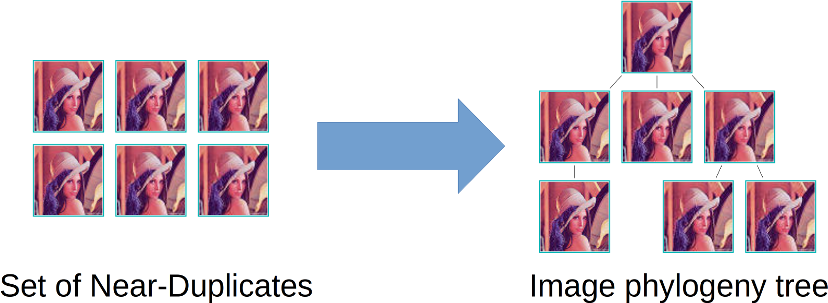
\includegraphics[width=0.8\textwidth]{set_to_tree.png}
  \end{center}
  Two parts during phylogeny tree reconstruction :
  \pause
  \begin{columns}
    \begin{column}{0.5\textwidth}
      \begin{block}{}
        \begin{itemize}
        \item Identify the root
        \end{itemize}
      \end{block}
      \pause
    \end{column}
    \begin{column}{0.5\textwidth}
      \begin{block}{}
        \begin{itemize}
        \item Estimate the rest of the tree
        \end{itemize}
      \end{block}
    \end{column}
  \end{columns}
\end{frame}

\begin{frame}
  \frametitle{Estimating the image phylogeny tree}

  \only<1> {
    \begin{block}{Visual Migration Map\footnotemark}
      \begin{itemize}
      \item Image manipulations are directional
      \item Parent-child relationship if manipulation directions are consistent
      \item Tree reconstruction using the longest path
      \end{itemize}
    \end{block}
    \footfullcitetext{kennedy2008internet}
  }
  \only<2> {
    \begin{center}
      \includegraphics<2>[scale=0.3]{vmm_directionnel}
    \end{center}
  }
\end{frame}

\begin{frame}
  \frametitle{Estimating the image phylogeny tree}
  \begin{block}{Image phylogeny tree \footnotemark[3] \footnotemark[4]}
    \begin{itemize}
    \item Extraction of a \textit{dissimilarity matrix}
    \item Tree reconstruction using a minimum spanning tree algorithm (e.g. Kruskal)
    \end{itemize}
  \end{block}
  \stepcounter{footnote}
  % \stepcounter{footnote}
  \footfullcitetext{dias2010first}
  \stepcounter{footnote}
  \footfullcitetext{dias2012image}
\end{frame}

% \begin{frame}
%   \frametitle{Estimation de la matrice de quantification primaire \footnotemark[6]}
%   \begin{block}{Principe de leur méthode}
%     Comparer l'histogramme de l'image originale et l'histogramme des images compressées avec des tables de quantification modèles puis compressées avec $Q_{f_2}$ et enfin garder la table pour laquelle la différence entre histogramme est la plus faible
%   \end{block}
%   \stepcounter{footnote}
%   \footfullcitetext{lukavs2003estimation}
% \end{frame}

% \begin{frame}
% \centering
% \begin{columns}[T] % align columns
% \begin{column}{.48\textwidth}
%   \begin{block}{Analyse des valeurs manquantes}
%     Artefacts distincts pour $Q_{f_1} > Q_{f_2}$ et $Q_{f_1} < Q_{f_2}$
%   \end{block}

%   \begin{block}{Limites}
%     \begin{itemize}
%     \item $Q_{f_1} = Q_{f_2}$
%     \item $Q_{f_1}$ est facteur de $Q_{f_2}$
%     \end{itemize}
%   \end{block}

%   % \hfill
%   \hspace*{-3.4mm}
%   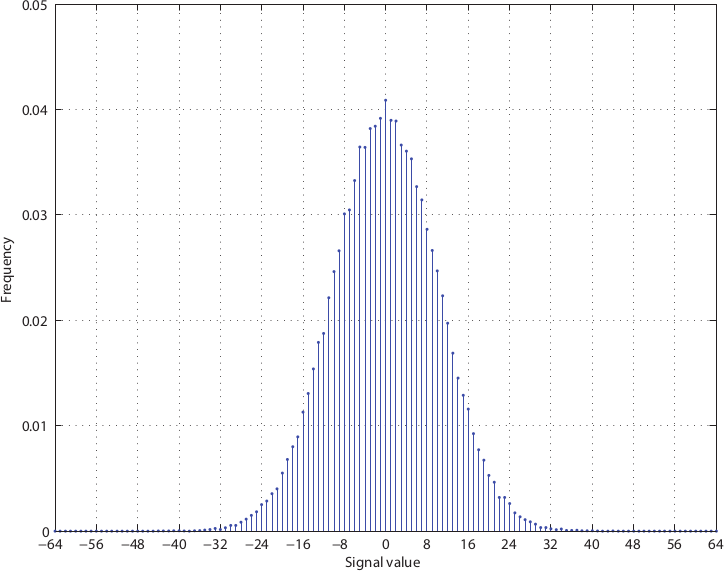
\includegraphics[height=0.475\textheight]{h1}
% \end{column}%
% \hfill%
% \begin{column}{.48\textwidth}
%   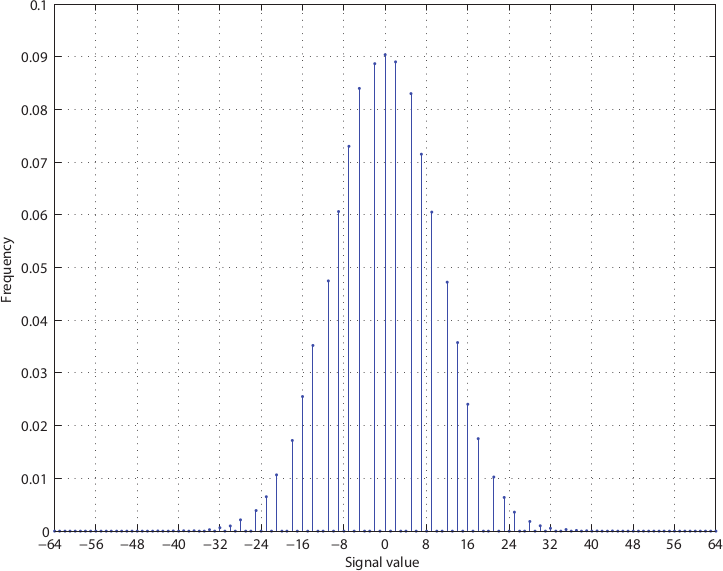
\includegraphics[height=0.475\textheight]{h2}
%   \hfill
%   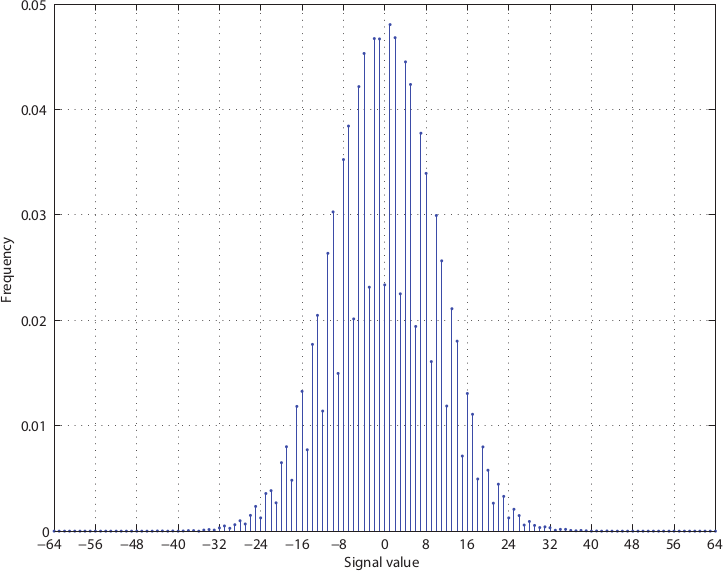
\includegraphics[height=0.475\textheight]{h3}
% \end{column}%
% \end{columns}
% \end{frame}


% \begin{frame}
%   \frametitle{Estimation de la matrice de compression primaire}
%   \begin{block}{Analyse des valeurs manquantes de l'histogramme}
%     Artefacts distincts pour $Q^{1} > Q^{2}$ et $Q^{1} < Q^{2}$
%   \end{block}
%   \pause
%   \begin{block}{Limites}
%     \begin{itemize}
%     \item $Q^{1} \neq Q^{2}$
%     \item $Q^{1}$ n'est pas facteur de $Q^{2}$
%     \end{itemize}
%   \end{block}
% \end{frame}


\section{Our method}

\begin{frame}
  \begin{block}{Goal}
    Reduce a complex image phylogeny tree reconstruction to a simple \textbf{parent-child relationship negation}
    % Réduction d'un problème de reconstruction d'un arbre de phylogénie à un problème de \textbf{négation de parenté}
  \end{block}
  \begin{block}{Solution}
    % Décision binaire entre deux images : ``Cette image est-elle le parent de cette autre image ?''
    Binary decision between two images : \textit{``Can this image be an ancestor of the other one?''}
  \end{block}
\end{frame}

\begin{frame}
  \frametitle{Our method}
  \begin{block}{Marker}
    A marker is a local or global feature extracted from the image. This marker shows that a particular transformation was applied to the image. This marker is passed on to the image child
  \end{block}
  \pause
  \begin{block}{Negation function}
    Let $f(I_{m},I_{n})$ be a function that for every image pair $(I_{m}, I_{n})$ detects every time there is one a marker visible in the image $I_m$ and not in its potential child $I_n$, thus proving that $I_m$ is not an ancestor of $I_n$
  \end{block}
  \pause
  \begin{block}{Theorem}
For all image pairs ($I_{m}$, $I_{n}$) in a set of near-duplicate images, if there is no marker proving that $I_m$ is not an ancestor of $I_n$ then there is a parent-child relationship between $I_{m}$ and $I_{n}$, $I_{m}$ $\to$ $I_{n}$, with $m < n$
  \end{block}
\end{frame}

\begin{frame}
  \frametitle{Diagram of our method}
  \begin{figure}[H]
    \centering
    % \begin{tikzpicture}[auto, distance=2in,sibling distance=.25in]
    \scalebox{0.61}{
      \begin{tikzpicture}[auto,node distance=2.1cm]

        \tikzstyle{every state}=[shape=rectangle,minimum width=1.1in,text width=1.1in, align=center,fill=blue!30]
        % \tikzstyle{every data}=[shape=circle,minimum width=1.3in,text width=1.3in, align=center,fill=blue!30]

        \node[draw=none,fill=none,minimum width=0.8in,text width=0.8in, align=center] (A) {Set of near-duplicates};
        \node[state] (B) [right=0.9cm of A] {DCT on each image};

        \node[draw=none,fill=none,minimum width=0.8in,text width=0.8in, align=center, right=0.9cm of B] (C) {DCT coefficients of each image};
        \node[state] (D) [right=0.9cm of C] {Extraction of the period of each DCT coefficient};

        \node[draw=none,fill=none,minimum width=0.8in,text width=0.8in, align=center, right=0.9cm of D] (E) {Extracted quantization table};
        \node[state] (F) [below=0.9cm of E] {Quality factor estimation};

        \node[draw=none,fill=none,minimum width=0.8in,text width=0.8in, align=center, left=0.9cm of F] (G) {$Q_f$ of each image};
        \node[draw=none,fill=none,minimum width=0.8in,text width=0.8in, align=center, below=0.3cm of G] (H) {Images};
        \node[state] (I) [left=0.9cm of G] {Ancestors estimation};

        \node[draw=none,fill=none,minimum width=0.8in,text width=0.8in, align=center, left=0.9cm of I] (J) {Parentage matrix};
        \node[state] (K) [left=0.9cm of J] {Tree reconstruction};

        \node[draw=none,fill=none,minimum width=0.8in,text width=0.8in, align=center, below=0.6cm of K] (L) {Unprocessed tree};
        \node[state] (M) [right=0.9cm of L] {Duplicates filtering};
        
        \node[draw=none,fill=none,minimum width=0.8in,text width=0.8in, align=center, right=0.9 of M] (N) {Image phylogeny tree};

        \path [->] (A) edge node[left] {} (B);
        \path [->] (B) edge node[left] {} (C);      
        \path [->] (C) edge node[left] {} (D);      
        \path [->] (D) edge node[] {} (E);      
        \path [->] (E) edge node[right] {} (F);      
        \path [->] (F) edge node[right] {} (G);      
        \path [->] (G) edge node[left] {} (I); 
        \path [->] (H) edge node[left] {} (I);
        \path [->] (I) edge node[left] {} (J);
        \path [->] (J) edge node[left] {} (K);
        \path [->] (K) edge node[left] {} (L);
        \path [->] (L) edge node[left] {} (M);
        \path [->] (M) edge node[left] {} (N);
      \end{tikzpicture}}
\end{figure}
\end{frame}

\begin{frame}
  \frametitle{$\widehat{q}(u,v)$ estimation}
  \begin{block}{How to get $\widehat{q}(u,v)$}
    \begin{itemize}
    \item Values of a quantized signal gather around the quantization step
    \item Delta between each peak of the autocorrelation of every DCT coefficient
    \end{itemize}
  \end{block}
  \centering
  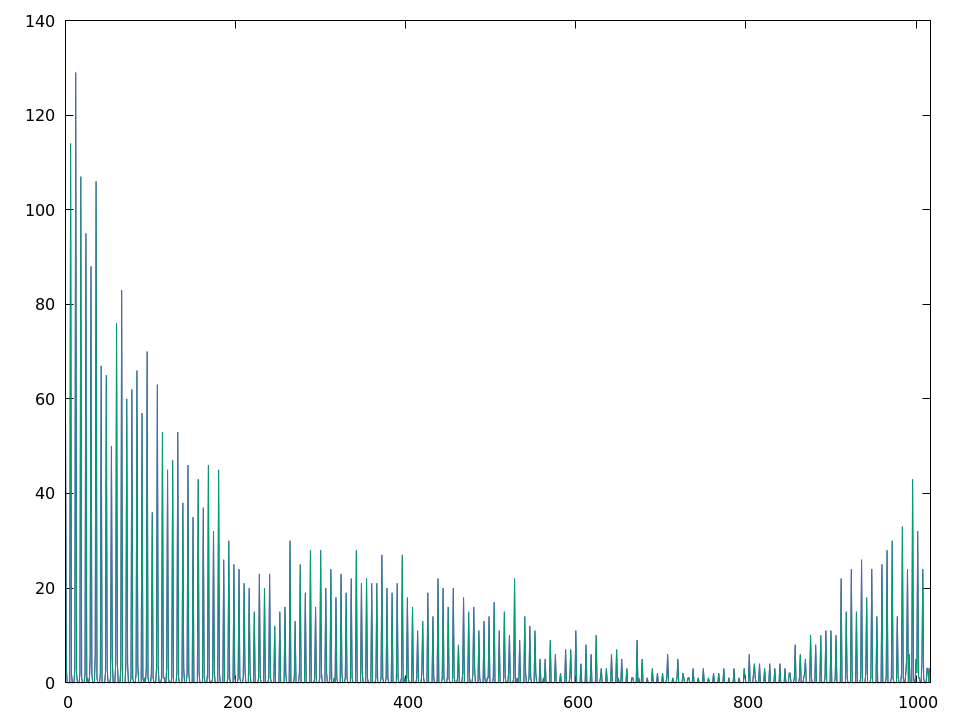
\includegraphics[width=0.5\linewidth]{signal.png}
  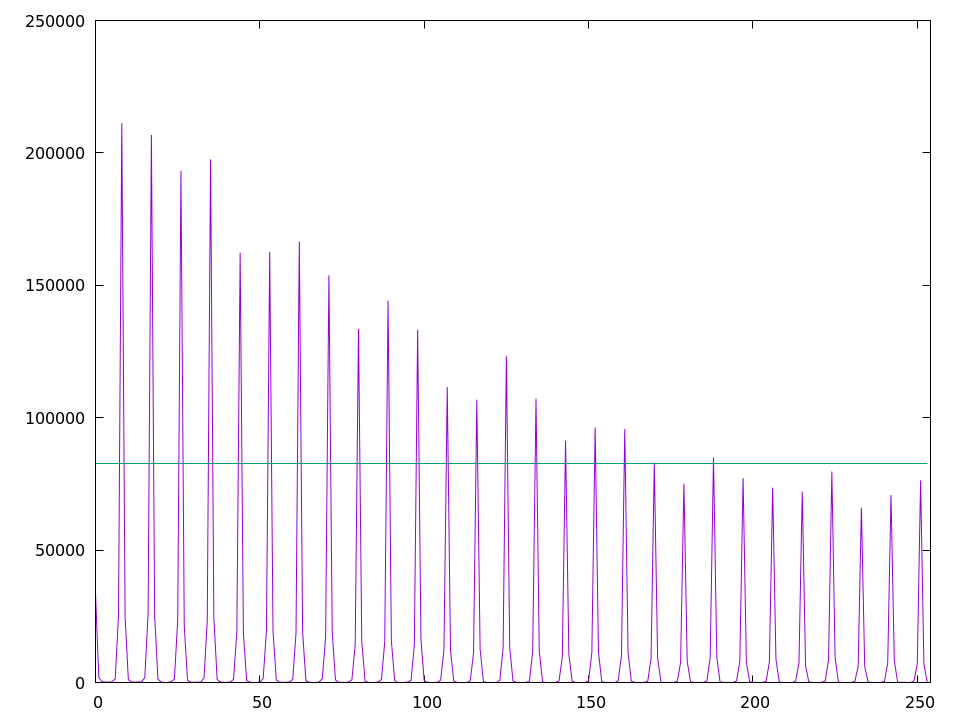
\includegraphics[width=0.5\linewidth]{autocorrelation.png}
\end{frame}

% \cellcolor{gray!25}

\begin{frame}
  \frametitle{$\widehat{q}(u,v)$ estimation}
  \begin{figure}
    \centering
    \begin{tabular}{|c|c|c|c|c|c|c|c|}
      \hline
      9 & 6 & 5 & 9 & 13 & 22 & 22 & 30 \\ \hline    
      6 & 6 & 8 & 10 & 14 & 16 & 30 & \cellcolor{gray!25} \\ \hline
      8 & 7 & 9 & 13 & 20 & 31 & \cellcolor{gray!25} & \cellcolor{gray!25} \\ \hline
      8 & 9 & 12 & 19 & 28 & \cellcolor{gray!25} & \cellcolor{gray!25} & \cellcolor{gray!25} \\ \hline
      10 & 12 & -1 & -1 & \cellcolor{gray!25} & \cellcolor{gray!25} & \cellcolor{gray!25} & \cellcolor{gray!25} \\ \hline
      12 & 13 & 30 & \cellcolor{gray!25} & \cellcolor{gray!25} & \cellcolor{gray!25} & \cellcolor{gray!25} & \cellcolor{gray!25} \\ \hline
      28 & 31 & \cellcolor{gray!25} & \cellcolor{gray!25} & \cellcolor{gray!25} & \cellcolor{gray!25} & \cellcolor{gray!25} & \cellcolor{gray!25} \\ \hline
      \cellcolor{gray!25} & \cellcolor{gray!25} & \cellcolor{gray!25} & \cellcolor{gray!25} & \cellcolor{gray!25} & \cellcolor{gray!25} & \cellcolor{gray!25} & \cellcolor{gray!25} \\ \hline
    \end{tabular}
    \caption{Example of a quantization table $\widehat{q}(u,v)$ returned by the period estimation}
    \label{periods1}
  \end{figure}
  \begin{block}{}
    Limited to the 35 first coefficients
  \end{block}
\end{frame}

% \begin{frame}
%   \frametitle{$\widehat{q}(u,v)$ estimation}
%   \centering
%   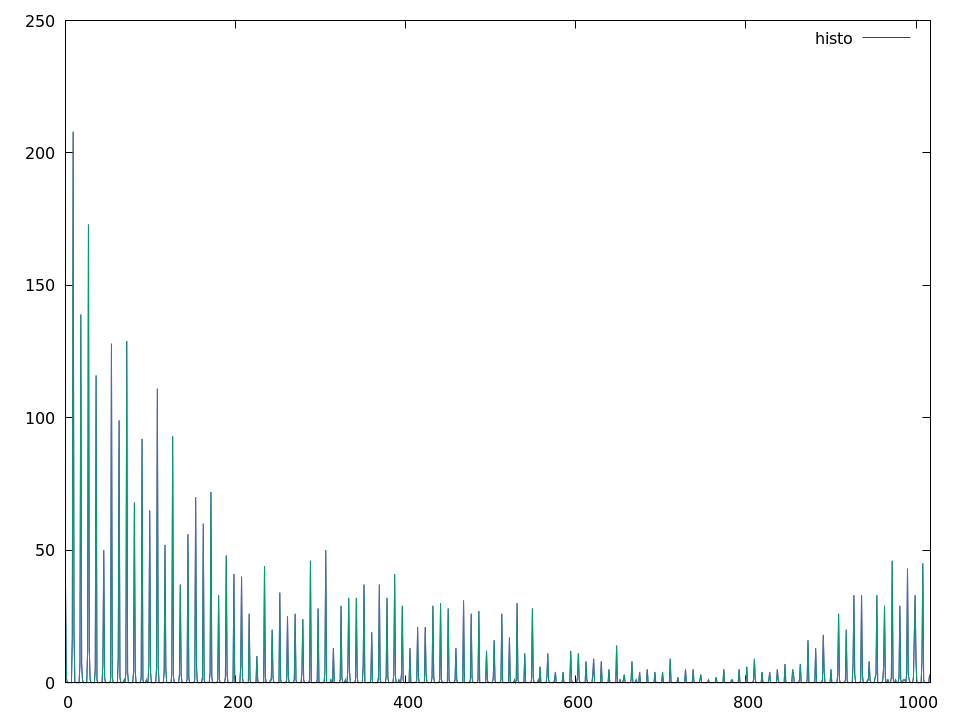
\includegraphics[width=0.45\linewidth]{histo0.png}
%   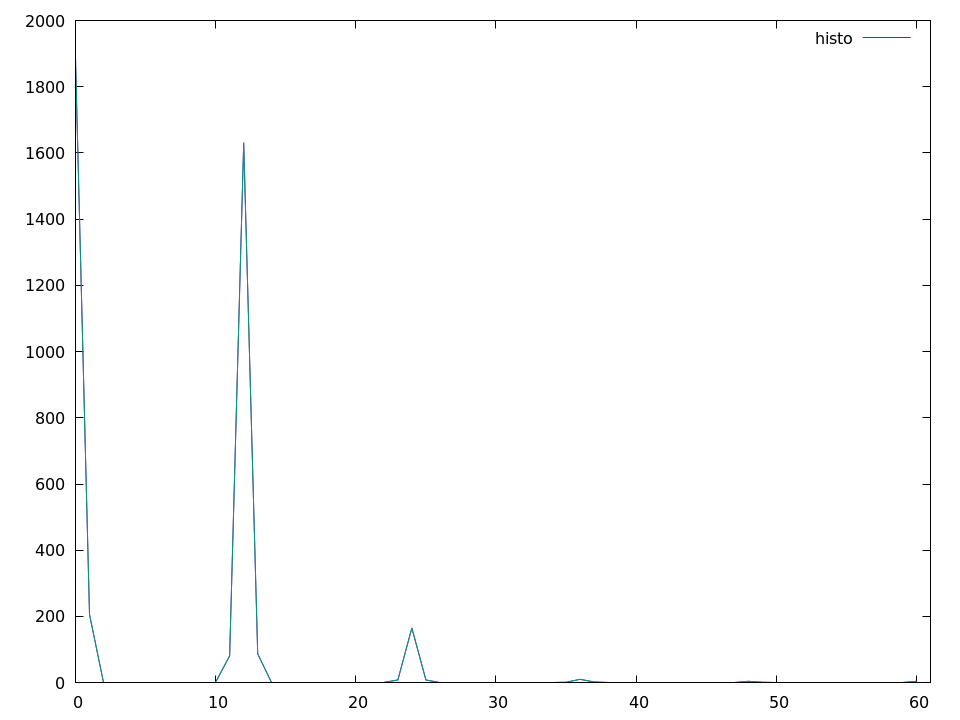
\includegraphics[width=0.45\linewidth]{histo18.png}


%   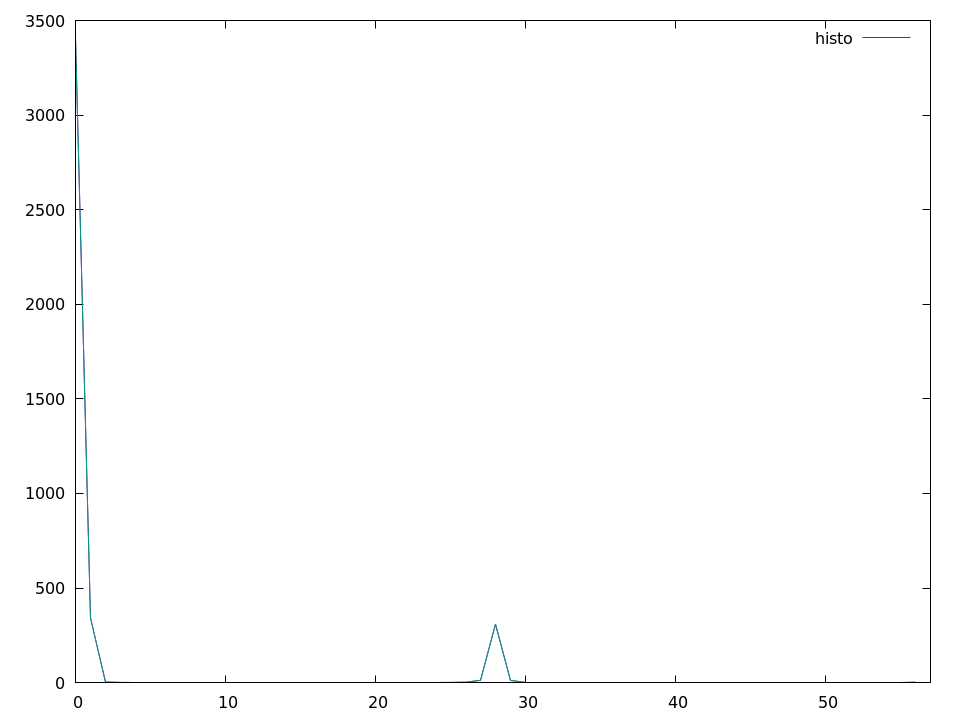
\includegraphics[width=0.45\linewidth]{histo31.png}
%   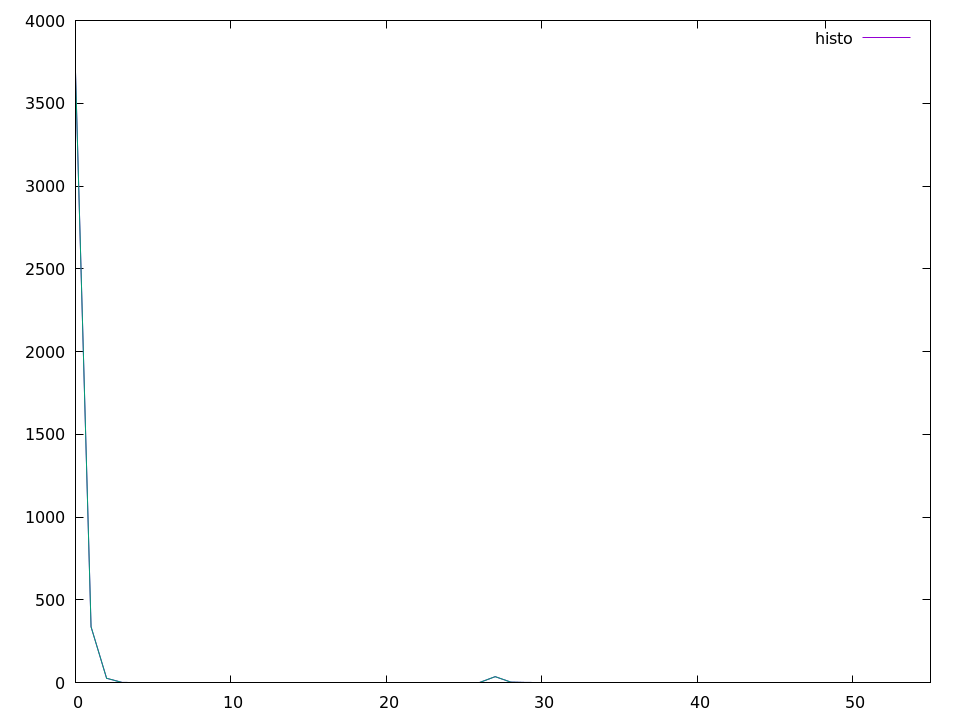
\includegraphics[width=0.45\linewidth]{histo40.png}
% \end{frame}

\begin{frame}
  \frametitle{Quality factor estimation}
  \begin{block}{Primary estimation}
    $$Q_f = argmin \sqrt{\sum\limits_{i=0}^{7}\sum\limits_{j=0}^{7}|\widehat{q}(i,j) - q_n(i,j)|^2}$$ where $q_n$ is a JPEG quantization table and $1 \leq n \leq 100$
    % Distance between $\widehat{q}(u,v)$ and quantization\_table(i), $1 \leq i \leq 100$ : $D_{euc}(P,Q) = \sqrt{\sum\limits_{i=1}^{d}|P_{i} - Q_{i}|^2}$
    % Calcul de distance entre $\widehat{q}(u,v)$ et table(i) : $D_{euc}(P,Q) = \sqrt{\sum\limits_{i=1}^{d}|P_{i} - Q_{i}|^2}$
  \end{block}
  \begin{block}{Secondary estimation}
    \begin{itemize}
    \item $\boldsymbol{if}\  Q_f < 50\  Q_s = 5000/Q_f\ \ \  \boldsymbol{else}\  Q_s = 200 - (Q_f \times 2) \ \ \ (1)$
    \item $q(u,v) = \frac{(q_{50}(u,v) \times Q_s) + 50}{100}\ \ with \ 1 \leq q(u,v) \leq 255\ \ \ \ \ \ \ \ \ (2)$
  \end{itemize}

    where $q_{50}$ is the reference JPEG quantization table for $Q_f = 50$.

  \end{block}
\end{frame}

\begin{frame}
  \frametitle{Quality factor estimation - example}
  % \centering
  \begin{figure}
    \hspace*{-1.5cm}
    \begin{subfigure}{0.6\linewidth}
      \centering
      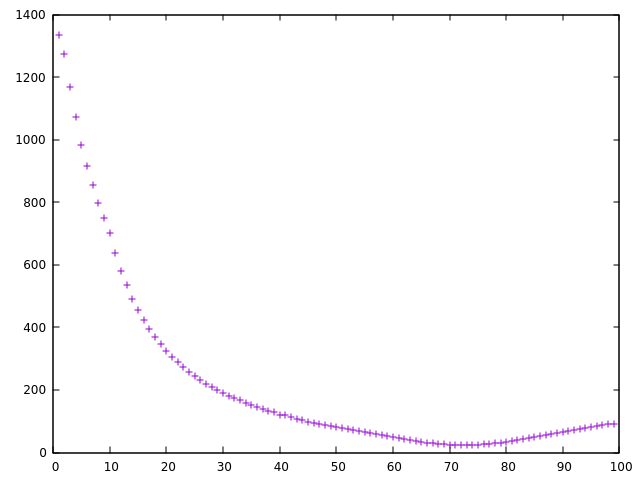
\includegraphics[width=0.95\linewidth]{distances.png}
    \caption{Plot of the distances between $\widehat{q}(u,v)$ and $q_n(u,v)$}
  \end{subfigure}%
  \hspace*{5mm}
    \begin{subfigure}{0.3\linewidth}
    % \scalebox{0.5}{
      % \centering
    %   \begin{tabular}{| C{0.58cm} | C{0.58cm} | C{0.58cm} | C{0.58cm} | C{0.58cm} | C{0.58cm} | C{0.58cm} | C{0.58cm} |}
    %     \hline
    %     32&24&28&28&36&48&98&144\\ \hline
    %     22&24&26&34&44&70&128&184\\ \hline
    %     20&28&32&44&74&110&156&190\\ \hline
    %     32&38&48&58&112&128&174&196\\ \hline
    %     48&52&80&102&136&162&206&224\\ \hline
    %     80&116&114&174&218&208&242&200\\ \hline
    %     102&120&138&160&206&226&240&206\\ \hline
    %     122&110&112&124&154&184&202&198\\ \hline
    %   \end{tabular}}
    % \caption{Quantization table for $Q_f = 25$}
    
    \vspace{-12mm}    

    \scalebox{0.5}{
      \begin{tabular}{| C{0.58cm} | C{0.58cm} | C{0.58cm} | C{0.58cm} | C{0.58cm} | C{0.58cm} | C{0.58cm} | C{0.58cm} |}
        \hline
        16&12&14&14&18&24&49&72\\ \hline
        11&12&13&17&22&35&64&92\\ \hline
        10&14&16&22&37&55&78&95\\ \hline
        16&19&24&29&56&64&87&98\\ \hline
        24&26&40&51&68&81&103&112\\ \hline
        40&58&57&87&109&104&121&100\\ \hline
        51&60&69&80&103&113&120&103\\ \hline
        61&55&56&62&77&92&101&99\\ \hline
      \end{tabular}}
    % \caption{Quantization table for $Q_f = 50$}
    \vspace{5mm}    
    
    \scalebox{0.5}{ 
      \begin{tabular}{| C{0.58cm} | C{0.58cm} | C{0.58cm} | C{0.58cm} | C{0.58cm} | C{0.58cm} | C{0.58cm} | C{0.58cm} |}
        \hline
        8&6&7&7&9&12&25&36\\ \hline
        6&6&7&9&11&18&32&46\\ \hline
        5&7&8&11&19&28&39&48\\ \hline
        8&10&12&15&28&32&44&49\\ \hline
        12&13&20&26&34&41&52&56\\ \hline
        20&29&29&44&55&52&61&50\\ \hline
        26&30&35&40&52&57&60&52\\ \hline
        31&28&28&31&39&46&51&50\\ \hline
      \end{tabular}}
    % \caption{Quantization table for $Q_f = 73$}

    \end{subfigure}
  \end{figure}
\end{frame}

\begin{frame}
  \frametitle{Quality factor estimation - example}
  Example for $u=0$ and $v=0$
  \begin{block}{Data}
    $\widehat{q}(0,0)=9,\ q_{50}(0,0)=16$
  \end{block}
  \begin{block}{Using equation (2)}
    $9=\frac{16\times Q_s + 50}{100}$, $\ \ \ Q_S = \frac{9\times 100 - 50}{16} = 53.125$
  \end{block}
  \begin{block}{Using equation (1)}
    $53.125 = 200 - (Q_f\times 2)$, $\ \ \ Q_f = \frac{200 - 53.125}{2} = 73.4375$
  \end{block}
  This process is repeated for every element in $\widehat{q}(u,v)$ and averaged to obtain an accurate estimation of $Q_f$
\end{frame}

% \begin{frame}
%   \frametitle{Estimation du facteur de qualité : estimation secondaire}
%   \begin{block}{Estimation secondaire}
%     Utilisation des formules 
%   \end{block}
%   \begin{block}{Avantages}
%     \begin{itemize}
%       \item Rapide
%       \item Précise
%     \end{itemize}
%   \end{block}
%   \begin{block}{Inconvénients}
%     $Q_f$ est nécessaire pour calculer $Q_f$
%   \end{block}

% \begin{equation}
%  Si\ \ \  Q_f < 50\ \ \ \  Q_s = 5000 / Q_f  \ \ sinon \ \ Q_s = 200 - (Q_f \times 2)
% \label{eqn:jpeg_1}
% \end{equation}

% \begin{equation}
% \begin{split}
%   q(u,v) = \frac{(base(u,v) \times Q_s) - 50}{100}\ \ \  avec\ \ \ 1 \leq q(u,v) \leq 255
% \end{split}
%   \label{eqn:jpeg_2}
% \end{equation}
% \end{frame}

\begin{frame}
  \frametitle{Ancestors estimation}
  \begin{block}{}
    JPEG compression is deterministic
  \end{block}
  \begin{block}{}
    JPEG compression is not transitive
  \end{block}
  \begin{block}{}
    The parent is one compression away from its children
  \end{block}
  \begin{block}{}
    Filtering images that can't be an ancestory
  \end{block}
  \begin{block}{}
    Binary decision
  \end{block}
\end{frame}

\begin{frame}
  \frametitle{Tree reconstruction}
  \begin{block}{}
    Binary matrix of size $n \times n$
  \end{block}
  \begin{block}{}
    Tree construction from the matrix
  \end{block}
\begin{figure}
  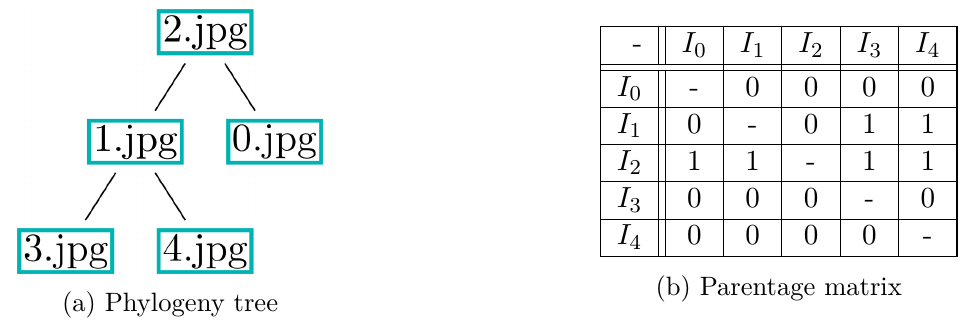
\includegraphics[width=.9\linewidth]{tree_table.png}
  % \centering
%   \subfloat[Arbre de phylogénie\label{Arbre de phylogenie}]{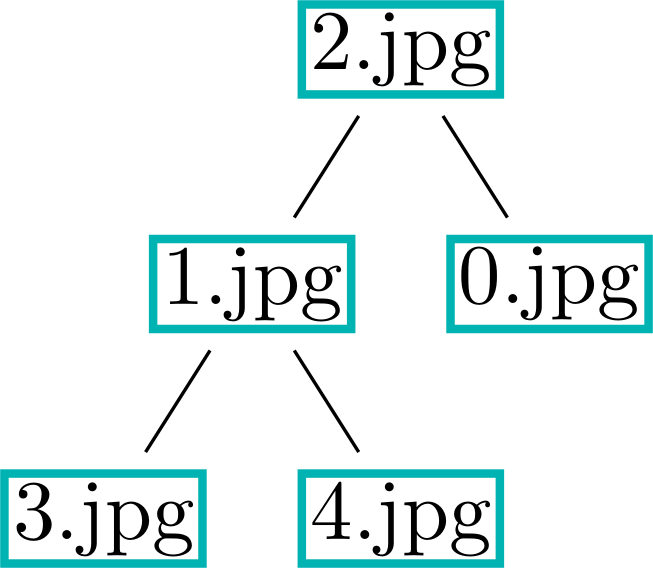
\includegraphics[width=.27\linewidth]{algo_tree.png}}
%   \subfloat[Matrice de parenté\label{fig:b}]{
%     \scalebox{0.75}{
%       \begin{tabular}{|r||c|c|c|c|c|}
%         \hline
%         - & $I_{0}$ & $I_{1}$ & $I_{2}$ & $I_{3}$ & $I_{4}$ \\ \hhline{|=::=|=|=|=|=|}
%         $I_{0}$ & - & 0 & 0 & 0 & 0 \\ \hline
%         $I_{1}$ & 0 & - & 0 & 1 & 1 \\ \hline
%         $I_{2}$ & 1 & 1 & - & 1 & 1 \\ \hline
%         $I_{3}$ & 0 & 0 & 0 & - & 0 \\ \hline
%         $I_{4}$ & 0 & 0 & 0 & 0 & - \\ \hline
%       \end{tabular} 
%     }
% }
%   \caption{A figure}
%   \label{fig:1}
\end{figure}

%   \begin{figure}
%       \centering
%       \subfloat{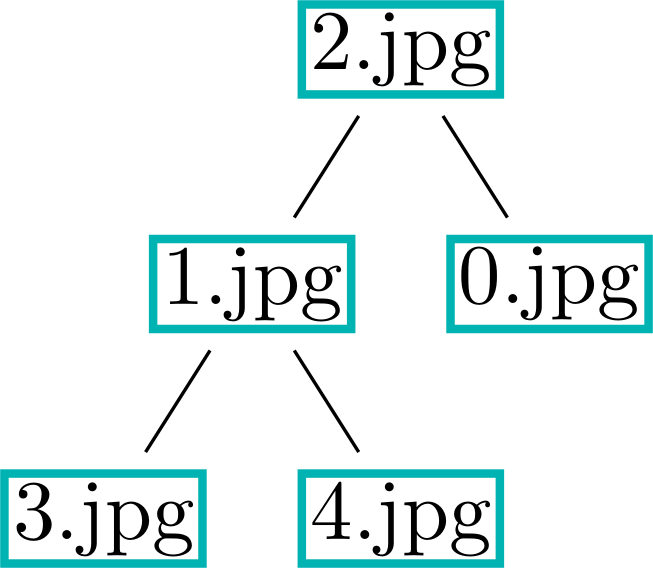
\includegraphics[width=.5\linewidth]{algo_tree.png}}
%       % \caption{Arbre de phylogénie}
%       % \label{algo_tree}
%     % \begin{subfigure}{.5\textwidth}
%       \centering
% \subfloat{
%       \begin{tabular}{|r||c|c|c|c|c|}
%         \hline
%         - & $I_{0}$ & $I_{1}$ & $I_{2}$ & $I_{3}$ & $I_{4}$ \\ \hhline{|=::=|=|=|=|=|}
%         $I_{0}$ & - & 0 & 0 & 0 & 0 \\ \hline
%         $I_{1}$ & 0 & - & 0 & 1 & 1 \\ \hline
%         $I_{2}$ & 1 & 1 & - & 1 & 1 \\ \hline
%         $I_{3}$ & 0 & 0 & 0 & - & 0 \\ \hline
%         $I_{4}$ & 0 & 0 & 0 & 0 & - \\ \hline
%       \end{tabular} 
%       % \caption{Matrice de parenté}
%       % \label{parentage_matrix}
%     % \end{subfigure}
% }
%     \caption{Une arbre de phylogénie et sa matrice de parenté.}
%     \label{parentage_tree}
%   \end{figure}

\end{frame}



% \begin{frame}
%   \frametitle{Points clés de notre approche}
%   \begin{block}{}
%     Réduction d'un problème de reconstruction d'un arbre de phylogénie à un problème de \textbf{négation de parenté}
%   \end{block}
%   \begin{block}{}
%     Facilement extensible
%   \end{block}
% \end{frame}

% \begin{frame}
%   \frametitle{Les marqueurs : facteur de qualité}
%   \centering
%   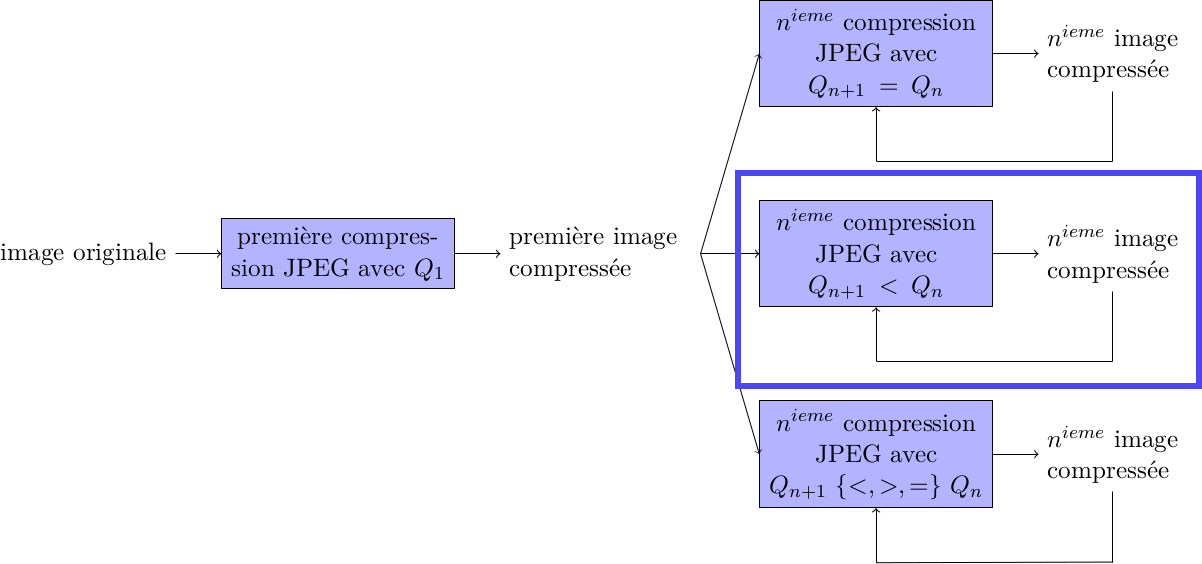
\includegraphics[width=0.8\linewidth]{qinf.png}
%   \begin{block}{}
%     Estimation du facteur de qualité
%   \end{block}
% \end{frame}

% \begin{frame}
%   \frametitle{Les marqueurs : valeurs manquantes dans l'histogramme des coefficients DCT}
%   \begin{block}{}
%     Les coefficients sont des multiples des valeurs de la table de quantification
    
%   \end{block}
%   \begin{figure}
%     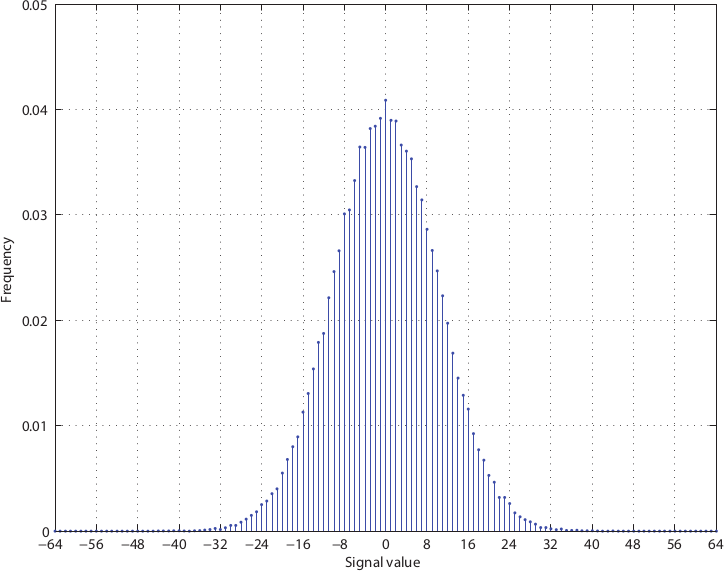
\includegraphics[width=0.5\linewidth]{h1.png}
%     % \caption{Image compressée une fois}
%     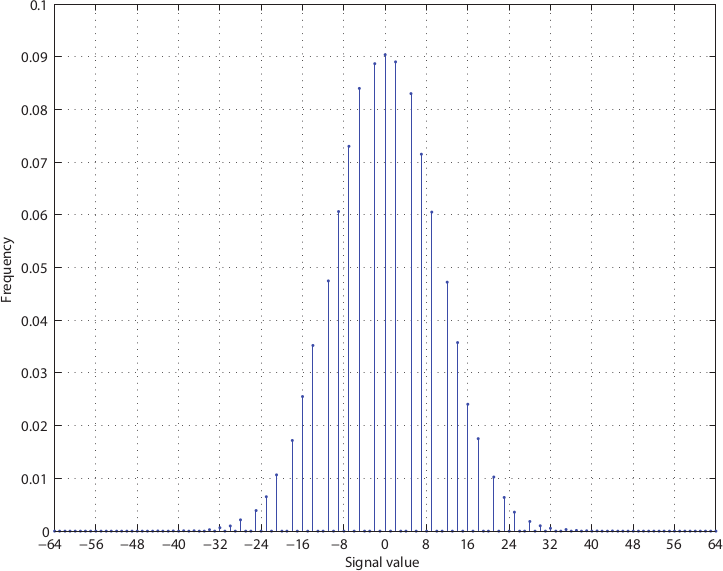
\includegraphics[width=0.5\linewidth]{h2.png}
%     % \caption{\ \ Image simplement compressée - Image doublement compressée, $Q_1 > Q_2$}
%   \end{figure}
% \vspace{-5mm}
% \scalebox{0.7}{
%   \hspace{15mm}
%   \textit{Image simplement compressée}
%   \hspace{18mm}
%   \textit{Image doublement compressée, $Q_1 > Q_2$}
% }  
% \end{frame}

\section{Results}
\begin{frame}
  \frametitle{On full trees}
  \begin{block}{}
    A very good estimation of $Q_f$
  \end{block}
  \begin{block}{}
    Metrics close to 100\%
  \end{block}
  \begin{block}{}
    A decreased accuracy with bigger trees
  \end{block}
\end{frame}

\begin{frame}
  \frametitle{On full trees}
  \centering
  \scalebox{0.85}{
  \begin{tabular}{|l||c|c|c|c|c|}
    \hline
     \backslashbox{Metric}{Dataset}             & \textbf{15 images} & \textbf{25 images} & \textbf{50 images} \\ \hhline{|=::=|=|=|}
    \textbf{\pbox{3.3cm}{Average $Q_f$ estimation error}} & 0.42 & 0.64 & 0.83 \\ \hhline{|=::=|=|=|}
    \textbf{roots}                                              & 95.83 & 88.88 & 84.72 \\ \hline
    \textbf{edges}                                              & 99.70 & 99.24 & 98.97 \\ \hline
    \textbf{leaves}                                             & 99.59 & 99.15 & 98.74 \\ \hline
    \textbf{ancestry}                                           & 99.44 & 96.88 & 96.96 \\ \hline
  \end{tabular}} 
\end{frame}

\begin{frame}
  \frametitle{Trees with a missing image}
  \begin{block}{}
    Bad root identification
  \end{block}
  \begin{block}{}
    Good estimation of the rest of the tree
  \end{block}
  \begin{block}{}
    Our method only detects parents
  \end{block}
\end{frame}

\begin{frame}
  \frametitle{Trees with a missing image}
  \centering
  \scalebox{0.9}{
    \begin{tabular}{c|c}
      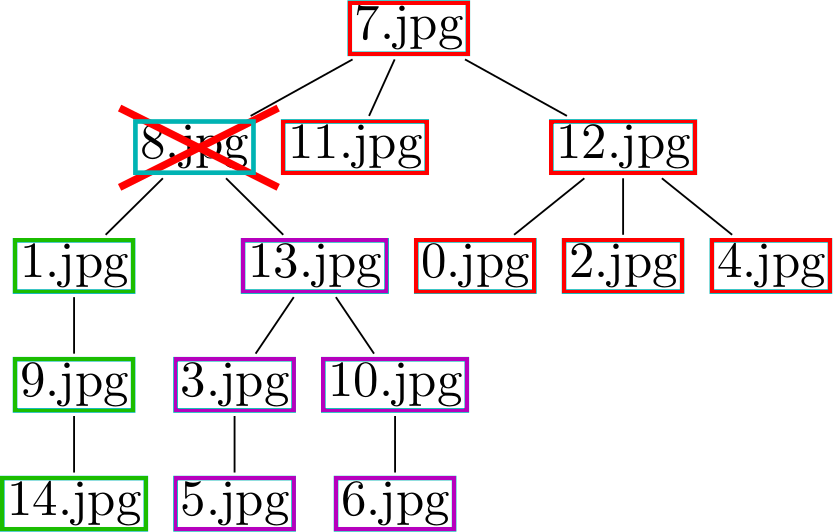
\includegraphics[width=.6\textheight]{tree_cross_color.png} & 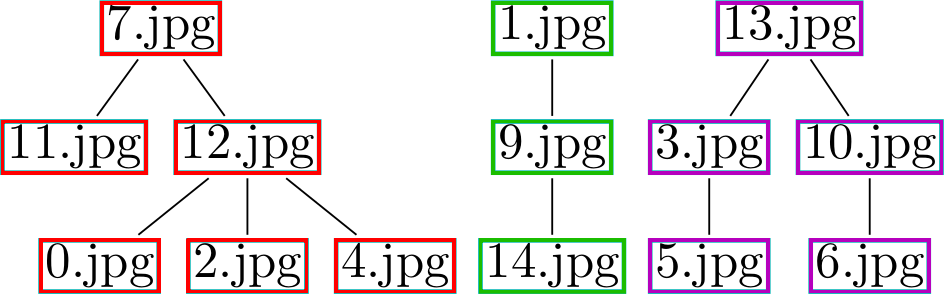
\includegraphics[width=.6\textheight]{3_trees_color.png} \\
    \end{tabular}
  }
\end{frame}

\begin{frame}
  \frametitle{Trees with color images}
  \begin{block}{}
    No change in our implementation
  \end{block}
  \begin{block}{}
    We used the luma component
  \end{block}
  \begin{block}{}
    Good results
  \end{block}
\end{frame}

\begin{frame}
  \frametitle{Trees with color images}
  \centering
  \scalebox{0.85}{
  \begin{tabular}{|l||c|c|c|c|c|}
    \hline
     \backslashbox{Metric}{Dataset}             & \textbf{15 images} & \textbf{25 images} & \textbf{50 images} \\ \hhline{|=::=|=|=|}
    \textbf{\pbox{3.3cm}{Average $Q_f$ estimation error}}         & 1.15  & 1.29  & 1.42  \\ \hhline{|=::=|=|=|}
    \textbf{roots}                                                      & 93.94 & 81.82 & 87.88 \\ \hline
    \textbf{edges}                                                      & 99.35 & 98.61 & 99.38 \\ \hline
    \textbf{leaves}                                                     & 99.62 & 98.66 & 99.78 \\ \hline
    \textbf{ancestry}                                                   & 98.79 & 94.13 & 98.82 \\ \hline
  \end{tabular}}
\end{frame}


  % \begin{block}{}
  %   Détection du parent direct très fiable
  % \end{block}
  % \pause
  % \begin{block}{}
  %   Mauvaise détection des parents éloignés
  % \end{block}
  % \pause
  % \begin{block}{}
  %   Arbre incomplet dans le cas d'images manquantes
  % \end{block}

\section{Conclusion}
\begin{frame}
  \frametitle{Conclusion - Perspectives}
  \begin{block}{Conclusion}
    \begin{itemize}
    \item A promising method with good results
    \item Limited to parents
    \end{itemize}
 \end{block}
 \begin{block}{Perspectives}
   \begin{itemize}
   \item Explore new distortions
   \item Discover new markers
   \end{itemize}
 \end{block}
\end{frame}

\begin{frame}
  \centering
\scalebox{3}{
 Questions ?
}
\end{frame}

\end{document}

